\documentclass[12pt,a4paper]{article}

\usepackage{amsfonts}
\usepackage{amsmath}
\usepackage{geometry}
\usepackage{graphicx}
\usepackage[dvipsnames,table]{xcolor}
\usepackage[subfolder,cleanup]{gnuplottex}
%\usepackage{amsthm}
%\usepackage{enumitem}
\usepackage{wrapfig}
\usepackage{subcaption}
%\usepackage{hyperref}
\usepackage{tikz}

\renewcommand\bottomfraction{.5}

\usetikzlibrary{%
	decorations.pathreplacing,%
 	decorations.pathmorphing%
}

\pgfdeclaredecoration{simple line}{initial}{
  \state{initial}[width=\pgfdecoratedpathlength-1sp]{\pgfmoveto{\pgfpointorigin}}
  \state{final}{\pgflineto{\pgfpointorigin}}
}

\tikzset{
   oshift/.style={decorate,decoration={simple line,raise=#1}}
}

\let\originalleft\left
\let\originalright\right
\renewcommand{\left}{\mathopen{}\mathclose\bgroup\originalleft}
\renewcommand{\right}{\aftergroup\egroup\originalright}

\newcommand{\diff}[3][]{\frac{d^{#1}#2}{d{#3}^{#1}}}
\newcommand{\pdiff}[3][]{\frac{\partial^{#1}#2}{\partial{#3}^{#1}}}

%\bibliographystyle{ieeetr}

\title{Position Sensing}
\author{Brady Metherall}
\date{October 28, 2019}

\newgeometry{margin=1in}
%\setlength\parindent{0pt}

\begin{document}
\maketitle

\section{Introduction}
We desire to be able to accurately determine the position of the end of a mechanical arm fixed to the ceiling. The arm is composed of a series of articulated rods connected together by joints with incremental encoders of a particular accuracy, and a tool attached to the free end. Each rod is of a given length, and the encoders measure the angle between adjacent rods relative to the initial conformation. A calibration at startup is required in order to determine the initial position. An example of such an arm is shown in Figure \ref{fig:scheme}.

\begin{figure}[tbp]
\centering
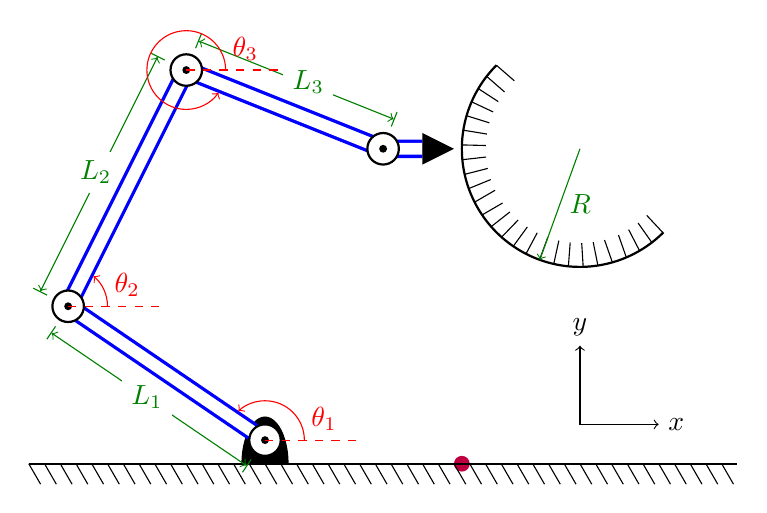
\begin{tikzpicture}
% Calibration point
\fill [purple] (2.5,0) circle (1mm);

% Ceiling
\draw [decorate,decoration={border,angle=-60,amplitude=3mm,segment length=2mm}] (-3,0) -- (6,0);
\draw [thick] (-3,0) -- (6,0);

% Car
\draw [decorate,decoration={border,angle=90,amplitude=3mm,segment length=1.88mm},domain=135:325] plot ({4+1.5*cos(\x)}, {4+1.5*sin(\x)});
\draw [thick,domain=135:315,samples=250] plot ({4+1.5*cos(\x)}, {4+1.5*sin(\x)});
\draw [->,Green] (4,4) -- (3.49,2.59) node [pos=0.5,anchor=west] {$R$};

% Anchor
\fill [domain=0:180] plot ({0.3*cos(\x)}, {0.6*sin(\x)});

% Lengths
\draw [|<->|,oshift=4mm,Green] (0,0.3) -- (-2.5,2) node [fill=white,pos=0.5,xshift=-2.5mm,yshift=-3mm] {$L_1$};
\draw [|<->|,oshift=4mm,Green] (-2.5,2) -- (-1,5) node [fill=white,pos=0.5,xshift=-4mm,yshift=2mm] {$L_2$};
\draw [|<->|,oshift=4mm,Green] (-1,5) -- (1.5,4) node [fill=white,pos=0.5,xshift=3mm,yshift=3.5mm] {$L_3$};

% Arms
\draw [blue,very thick,double,double distance=1.5mm] (0,0.3) -- (-2.5,2) -- (-1,5) -- (1.5,4) -- (2,4);
\fill (2,3.8) -- (2,4.2) -- (2.4,4) -- cycle;

% Joints
\draw [thick,fill=white] (0,0.3) circle (0.2);
\draw [thick,fill=white] (-2.5,2) circle (0.2);
\draw [thick,fill=white] (-1,5) circle (0.2);
\draw [thick,fill=white] (1.5,4) circle (0.2);
\fill (0,0.3) circle (0.05);
\fill (-2.5,2) circle (0.05);
\fill (-1,5) circle (0.05);
\fill (1.5,4) circle (0.05);

% Angles
\draw [red,dashed] (0,0.3) -- (1.25,0.3) node [pos=0.6,anchor=south] {$\theta_1$};
\draw [red,dashed] (-2.5,2) -- (-1.25,2) node [pos=0.6,anchor=south] {$\theta_2$};
\draw [red,dashed] (-1,5) -- (0.25,5) node [pos=0.6,anchor=south] {$\theta_3$};
\draw [->,red] (0.5,0.3) arc (0:132.5:0.5);
\draw [->,red] (-2,2) arc (0:50:0.5);
\draw [->,red] (-0.5,5) arc (0:325:0.5);

% Coordinates
\draw [<->,thin] (5,0.5) -- (4,0.5) -- (4,1.5);
\node [anchor=west] at (5,0.5) {$x$};
\node [anchor=south] at (4,1.5) {$y$};

\end{tikzpicture}
\caption{Schematic of a 3-rod arm. The final link is the attached tool. The arc and lower surface represent the work piece and ceiling respectively---the coordinate system has been inverted for convenience. The plum coloured dot represents a known calibration point.}
\label{fig:scheme}
\end{figure}

\section{Model}
\label{sec:model}
In order to simplify the modelling process, we shall assume the rods are rigid and have 0 width so they can be treated as line segments. Additionally, for convenience, we shall take the mount point of the arm to be the origin with the positive $y$ direction to be opposite the ceiling. \\

Furthermore, we shall assume the work piece is half of a circle centred at (1m,1m), with diameter 0.75m and oriented towards the origin, and that the tool at the end of the arm is 0.15m. For ease of the mathematics we will not explicitly model the tool. We must also work under the constraints that each rod can be no longer than 1m, and the error in the position of the tool must be less than half an inch. \\

As we are interested in the end of a series of rods attached together at various angles, it is natural to examine the system geometrically. If we measure the angles with respect to the positive $x$ axis then the position of the end of the arm is simply
\begin{align}
x &= \sum_{i=1}^N L_i \cos \theta_i, & y &= \sum_{i=1}^N L_i \sin \theta_i,
\label{eq:model}
\end{align}
where $L_i$ is the length of the $i$th rod, $\theta_i$ is the absolute angle of the $i$th joint, and $N$ is the number of rods in the arm.

\section{Results}
\label{sec:results}

\begin{wraptable}{R}{9.5cm}
\vspace{-11mm}
\centering
\begin{tabular}{cccc}
Reading 1 & Reading 2 & Reading 3 & Reading 4 \\
\noalign{\global\arrayrulewidth=1.25pt}\hline
\rowcolor{gray!10}
-0.07420 & \ 0.07420 & -0.04497 & -0.00179 \\
-0.07420 & \ 0.02742 & \ 0.02853 & -0.07487 \\
\rowcolor{gray!10}
-0.02412 & -0.16026 & \ 0.27843 & -0.27794 \\
\ 0.07272 & \ 1.20678 & \ 4.78410 & \ 1.30220 \\
\rowcolor{gray!10}
-0.71895 & \ 0.71895 & -0.52670 & -0.15747 \\
\hline
\end{tabular}
\caption{Sample data from the encoders. Rows 1--3 correspond to an initial state of a regular pentagon, rows 4 and 5 purposely have unphysical initial conformations.}
\label{tab:data}
\vspace{-10mm}
\end{wraptable}

With our geometric model defined we are ready to investigate the nature of the model.

\subsection{Calibration}
Given the sample data in Table \ref{tab:data} for a 4-rod arm, we wish to be able to determine the absolute angles, $\theta_i$---we must first calibrate the system. To do so we shall touch the end of the arm to a known calibration point, then turn on the arm. We assume this point is on the ceiling 1m from the mount point of the arm, however, the actual location is irrelevant. This gives us the equations
\begin{align}
\sum_{i=1}^4 L_i \cos \varphi_i &= 1, & \sum_{i=1}^4 L_i \sin \varphi_i &= 0,
\label{eq:angularstart}
\end{align}
where $\varphi_i$ is the, to be determined, absolute angle at startup of the $i$th joint. Now, by moving the arm while keeping the end on the calibration point we obtain the additional equations
\begin{align}
\sum_{i=1}^4 L_i \cos \left( \varphi_i + \delta_i \right) &= 1, & \sum_{i=1}^4 L_i \sin \left( \varphi_i + \delta_i \right) &= 0,
\label{eq:angulardiff}
\end{align}
where $\delta_i$ is the angular difference of the $i$th joint, which are the partial sums of the measurements from the encoders. By combining \eqref{eq:angularstart} and \eqref{eq:angulardiff} we obtain a system of four equations and four unknowns, $\varphi_i$, thus we will obtain a unique solution\footnote{Assuming $0 \leq \theta_i < 2 \pi$.} and can determine the absolute angles of the starting position, and therefore the absolute angle at any later time from the readings of the encoders. Both typical and unphysical measurements are shown in Table \ref{tab:data}. The solutions of \eqref{eq:angularstart} and \eqref{eq:angulardiff} using the data from Table \ref{tab:data} are shown in Figure \ref{fig:shapes}, we find the expected result of a regular pentagon in the case of the first three rows, and unphysical solutions in the case of the last two rows. \\

\begin{figure}[tbp]
\centering
\begin{gnuplot}[terminal=epslatex, terminaloptions={color size 4in,3.2in lw 3}]
#load '/home/brady/Templates/Blues.p'
set grid
set size ratio -1
set key at 1,0.75
set key width -2
set xl '$x$'
set yl rotate by 0 '$y$'
set xtics 0.5
set ytics 0.4
plot 'Shape.dat' u 1:2 dt 5 w l t 'Calibration', \
'Shape.dat' u 3:4 w l t 'Data set 1', \
'Shape.dat' u 5:6 w l t 'Data set 2', \
'Shape.dat' u 7:8 w l t 'Data set 3'
\end{gnuplot}
\caption{By solving \eqref{eq:angularstart} and \eqref{eq:angulardiff} using data from Table \ref{tab:data} we find the starting configuration of a regular pentagon in the case of the first three data sets. The solutions to data sets 4 and 5 are unphysical as expected and are not shown.}
\label{fig:shapes}
\end{figure}

This process can easily be generalized to any number of rods. In the $n$-rod case we require $n$ equations to determine the starting configuration. Since each perturbation after startup yields two additional equations, we simply need $\lceil \frac{n-2}{2} \rceil$ perturbations after the initial state in order to calibrate.

\subsection{Range of Motion of a 2-Rod Arm}
\label{sec:range}
We shall now examine where on the work surface a 2-rod arm can reach. Ideally, the tool will be able to reach every spot on the work piece at every angle. Thus, the end of the arm needs to reach every point within a shell of 0.15m from the work piece, as depicted in Figure \ref{fig:angle}. To accomplish this, we prescribe a particular $(x,y)$ coordinate and numerically solve \eqref{eq:model}, if no solution is found the position is unreachable. On the other hand, if a solution is found, we must confirm it is a physical solution---that is, the second rod does not penetrate the work piece\footnote{We do not have to consider the case of the first rod penetrating the work piece as it cannot reach it.}. \\

\begin{wrapfigure}{R}{0.5\textwidth}
\centering
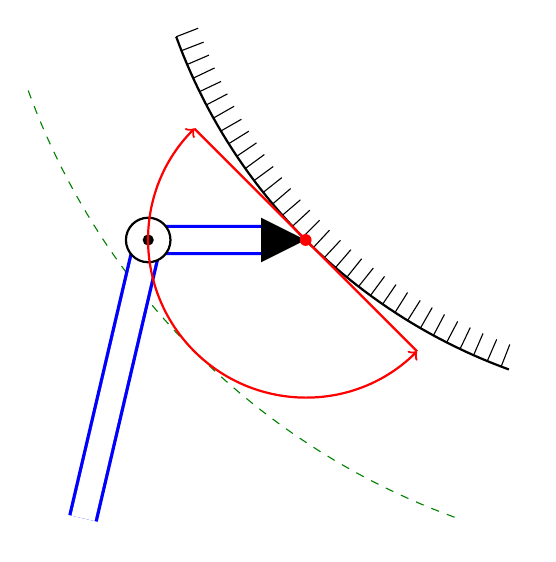
\begin{tikzpicture}[x=0.707cm,y=0.707cm]
% Car
\draw [decorate,decoration={border,angle=90,amplitude=3mm,segment length=1.895mm},domain=200:252] plot ({10/sqrt(2) + 10*cos(\x)}, {10/sqrt(2) + 10*sin(\x)});
\draw [thick,domain=200:250,samples=250] plot ({10/sqrt(2) + 10*cos(\x)}, {10/sqrt(2) + 10*sin(\x)});

% Green outline
\draw [domain=200:250,samples=250,Green,dashed] plot ({10/sqrt(2) + 12.82842*cos(\x)}, {10/sqrt(2) + 12.82842*sin(\x)});

% Arms
\draw [blue,very thick,double,double distance=3mm] (-4,-5) -- (-2.82842,0) -- (-0.7,0);
\fill (-0.8,-0.4) -- (-0.8,0.4) -- (0,0) -- cycle;

% Joint
\draw [thick,fill=white] (-2.82842,0) circle (0.4);
\fill (-2.82842,0) circle (0.1);

% Red semicircle
\fill [red] (0,0) circle (0.75mm); % Dot
\draw [thick,red] (-2,2) -- (2,-2); % Line
\draw [thick,red,<->] (-2,2) arc (135:315:2.82842); % Arc
\end{tikzpicture}
\caption{In order for the tool to reach every point on the work piece at every angle the last link must be able to reach all points within the length of the tool from the work piece.}
\label{fig:angle}
\end{wrapfigure}

We proceed by first parameterizing the second rod as
\begin{align}
\mathbf{s}(t) = L_1
\begin{pmatrix}
\cos \theta_1 \\
\sin \theta_1
\end{pmatrix}
+ L_2
\begin{pmatrix}
\cos \theta_2 \\
\sin \theta_2
\end{pmatrix}
t.
\label{eq:param}
\end{align}
We can now substitute \eqref{eq:param} into the equation of the work piece,
\begin{align}
(x-1)^2 + (y-1)^2 = R^2.
\label{eq:circ}
\end{align}
If $t$ has a real solution between 0 and 1 then the second rod intersects the work piece and the solution is not physical. If $t$ has real solutions outside of this range the rod is pointed at the work piece but does not pass through it. And finally, if $t$ has complex conjugate solutions the rod is not pointed towards the work piece\footnote{See Appendix \ref{sec:geo}.}. \\

We first carry out this process in the case $L_1 = 1$, and $L_2 = 0.6$---the results are shown in Figure \ref{fig:long}. We can see that the farthest points around the work piece are not reachable, and also that since $L_2 > 0.475$ the arm cannot reach parts directly below the work piece since the first rod is against the ceiling, and the second rod is too long. \\

Knowing this limitation, we repeat the same process after shortening the second rod to $L_2 = 0.475$, the result is shown in Figure \ref{fig:short}. As expected the arm is now able to reach the area directly below the work piece. However, as with the first trial the arm is not quite long enough to reach the farthest points around the work piece. \\

From these two trials it seems it is not possible to reach the entire work piece at all angles in the 2-rod case. However, by adding a third rod this is unlikely to be a problem, although the problem becomes more difficult computationally since the system becomes under determined.

\begin{figure}[tbp]
\centering
\begin{subfigure}{0.5\textwidth}
\begin{gnuplot}[terminal=epslatex, terminaloptions={color size 3.2in,3.2in lw 3}]
load './PlotStyle.p'
p 'Total.dat' u 1:2 pt 7 ps .5 lc rgb 'red' t 'Unreachable', \
'Long.dat' u 1:2 pt 7 ps 0.5 lc rgb 'web-green' t 'Reachable', \
sqrt(0.6**2 - (x-1)**2) dt 5 t 'Minimum Reach'
\end{gnuplot}
\vspace{-8mm}
\caption{$L_1 = 1$, $L_2 = 0.6$.}
\label{fig:long}
\end{subfigure}%
\begin{subfigure}{0.5\textwidth}
\begin{gnuplot}[terminal=epslatex, terminaloptions={color size 3.2in,3.2in lw 3}]
load './PlotStyle.p'
p 'Total.dat' u 1:2 pt 7 ps .5 lc rgb 'red' t 'Unreachable', \
'Short.dat' u 1:2 pt 7 ps 0.5 lc rgb 'web-green' t 'Reachable', \
sqrt(1.475**2 - x**2) dt 5 t 'Maximum Reach'
\end{gnuplot}
\vspace{-8mm}
\caption{$L_1 = 1$, $L_2 = 0.475$.}
\label{fig:short}
\end{subfigure}
\caption{Reach of a 2-rod arm.}
\label{fig:reach}
\end{figure}

\subsection{Tolerance}
\label{sec:tol}
As mentioned in Section \ref{sec:model}, the encoders must be accurate enough to determine the position of the end of the arm within half an inch. The positional error can the be calculated as half of the difference of the maximum error in either direction:
\begin{align*}
x_\text{err} = \frac{1}{2} \left| \sum_{i=1}^N L_i \left( \cos \left( \theta_i + \sum_{j=1}^i \phi_j^\text{tol} \right) - \cos \left( \theta_i - \sum_{j=1}^i \phi_j^\text{tol} \right) \right) \right|,
\end{align*}
where $\phi_j^\text{tol}$ is the angular tolerance of the $j$th encoder. This expression can be greatly simplified using trigonometric identities and noting that $\phi_j^\text{tol} \ll 1$. Using the same procedure for $y_\text{err}$ we find 
\begin{align}
x_\text{err} &= \left| \sum_{i=1}^N L_i \sin \theta_i \sum_{j=1}^i \phi_j^\text{tol} \right|, & y_\text{err} &= \left| \sum_{i=1}^N L_i \cos \theta_i \sum_{j=1}^i \phi_j^\text{tol} \right|.
\end{align}

By taking the partial derivatives we can find how the errors propagate along the arm depending on our choices of lengths and accuracies. With respect to the $k$th rod we find the errors vary as
\begin{align}
\pdiff{x_\text{err}}{L_k} &= \left| \sin \theta_k \sum_{j=1}^k \phi_j^\text{tol} \right|, & \pdiff{y_\text{err}}{L_k} &= \left| \cos \theta_k \sum_{j=1}^k \phi_j^\text{tol} \right|.
\end{align}
As the error induced by the $k$th rod scales linearly with the partial sum of the accuracies, it is more beneficial to have longer rods closer to the ceiling than the free end. Similarly,
\begin{align}
\pdiff{x_\text{err}}{\phi_k^\text{tol}} &= \left| \sum_{i=k}^N L_i \sin \theta_i \right|, & \pdiff{y_\text{err}}{\phi_k^\text{tol}} &= \left| \sum_{i=k}^N L_i \cos \theta_i \right|,
\end{align}
for the encoders' accuracies. In the opposite case to the lengths, the encoders closer to the ceiling propagate their errors through the entire arm. Therefore, it is preferable to have the encoders sorted in decreasing accuracy order, that is, the most accurate first and the least accurate last. Finally, in order to satisfy the accuracy requirement, it must be that
\begin{align}
\frac{1}{2} \text{in} \geq \sqrt{x_\text{err}^2 + y_\text{err}^2}.
\label{eq:acc}
\end{align}

\section{Conclusion}
To accurately measure the end of a mechanical arm given the relative changes in the angles, we developed a geometric model for the rods composing the arm. Based on our findings in Section \ref{sec:results}, we have the following recommendation for assembling such a mechanical arm. \\

In Section \ref{sec:range} we established that a 3-rod arm would likely be sufficient to reach all locations of the work piece at all angles. Furthermore, in Section \ref{sec:tol} we found an expression for the accuracy of the arm. In the case of a 3-rod arm, \eqref{eq:acc} can be simplified to
\begin{align}
0.0127\text{m} \geq  L_1  \phi_1^\text{tol} +  L_2 \left( \phi_1^\text{tol} + \phi_2^\text{tol} \right) + L_3 \left( \phi_1^\text{tol} + \phi_2^\text{tol} + \phi_3^\text{tol} \right).
\label{eq:simptol}
\end{align}
Let us---somewhat arbitrarily---assign the lengths of the rods: $L_1 = 1$m to maximize the length of the first rod. And $L_2 = L_3 = 0.4$m to ensure the arm is able to reach the farthest areas of the work piece while still able to maneuver from one side of the work piece to the other. \\

If we now assume that an encoder with twice the angular resolution is twice the price we can estimate the cost of the encoders as
\begin{align}
C = \alpha \left( \frac{1}{\phi_1^\text{tol}} + \frac{1}{\phi_2^\text{tol}} + \frac{1}{\phi_3^\text{tol}} \right),
\label{eq:cost}
\end{align}
where $C$ is the cost of the encoders, and $\alpha$ is how the price scales. By minimizing \eqref{eq:cost} while constrained to \eqref{eq:simptol}, we find that the optimum is when $\phi_2^\text{tol} = 1.5\phi_1^\text{tol}$, $\phi_3^\text{tol} = 2.1213\phi_1^\text{tol}$, and $\phi_1^\text{tol} \approx 3.300 \times 10^{-3}$rad. \\

All of the analysis has been done in two dimensions, however, our work piece has a length that we have not considered. Our model can be adjusted to account for the additional dimension by considering spherical coordinates instead of polar, and including further degrees of freedom in the encoders. This generalization, however, is non-trivial. Thus, it is our suggestion to mount the arm to a slider fastened to the ceiling to allow motion in the $z$ direction.

\appendix
\section{Geometric Constraint}
\label{sec:geo}
Solving the quadratic in $t$ obtained by substituting \eqref{eq:param} into \eqref{eq:circ} yields
\begin{align*}
t &= \frac{\sin \left(\theta _2\right)+\cos \left(\theta _2\right)-L_1 \cos \left(\theta _1-\theta _2\right)\pm\sqrt{\Delta}}{L_2},
\end{align*}
where $\Delta$, the discriminant, is
\begin{align*}
\Delta &= -L_1^2 \sin ^2\left(\theta _1-\theta _2\right)+2 L_1 \sin \left(\theta _1-\theta _2\right) \left(\cos \left(\theta _2\right)-\sin \left(\theta _2\right)\right)+\sin \left(2 \theta _2\right)+R^2-1.
\end{align*}


%\bibliography{Ref}

\end{document}




